

\documentclass[twoside,twocolumn]{article}

\usepackage{blindtext} % Package to generate dummy text throughout this template 
\usepackage{graphicx}
\usepackage[sc]{mathpazo} % Use the Palatino font
\usepackage[T1]{fontenc} % Use 8-bit encoding that has 256 glyphs
\linespread{1.05} % Line spacing - Palatino needs more space between lines
\usepackage{microtype} % Slightly tweak font spacing for aesthetics

\usepackage[english]{babel} % Language hyphenation and typographical rules

\usepackage[hmarginratio=1:1,top=32mm,columnsep=20pt]{geometry} % Document margins
\usepackage[hang, small,labelfont=bf,up,textfont=it,up]{caption} % Custom captions under/above floats in tables or figures
\usepackage{booktabs} % Horizontal rules in tables

\usepackage{lettrine} % The lettrine is the first enlarged letter at the beginning of the text

\usepackage{enumitem} % Customized lists
\setlist[itemize]{noitemsep} % Make itemize lists more compact

\usepackage{abstract} % Allows abstract customization
\renewcommand{\abstractnamefont}{\normalfont\bfseries} % Set the "Abstract" text to bold
\renewcommand{\abstracttextfont}{\normalfont\small\itshape} % Set the abstract itself to small italic text

\usepackage{titlesec} % Allows customization of titles
\renewcommand\thesection{\Roman{section}} % Roman numerals for the sections
\renewcommand\thesubsection{\roman{subsection}} % roman numerals for subsections
\titleformat{\section}[block]{\large\scshape\centering}{\thesection.}{1em}{} % Change the look of the section titles
\titleformat{\subsection}[block]{\large}{\thesubsection.}{1em}{} % Change the look of the section titles

\usepackage{fancyhdr} % Headers and footers
\pagestyle{fancy} % All pages have headers and footers
\fancyhead{} % Blank out the default header
\fancyfoot{} % Blank out the default footer
\fancyhead[C]{Virtualizacion y contenedores $\bullet$ Mayo 2019 $\bullet$ } % Custom header text
\fancyfoot[RO,LE]{\thepage} % Custom footer text

\usepackage{titling} % Customizing the title section

\usepackage{hyperref} % For hyperlinks in the PDF

%----------------------------------------------------------------------------------------
%	TITLE SECTION
%----------------------------------------------------------------------------------------

\setlength{\droptitle}{-4\baselineskip} % Move the title up

\pretitle{\begin{center}\Huge\bfseries} % Article title formatting
\posttitle{\end{center}} % Article title closing formatting
\title{Virtualizacion y Contenedores} % Article title
\author{Andre Reinoso, Samuel Nuñez, Andre De la Barra y David Damian}
\date{\today} % Leave empty to omit a date
\renewcommand{\maketitlehookd}{%
\begin{abstract}
\noindent ACA VA EL ABSTRACT
\end{abstract}
}

%----------------------------------------------------------------------------------------

\begin{document}

% Print the title
\maketitle

%----------------------------------------------------------------------------------------
%	ARTICLE CONTENTS
%----------------------------------------------------------------------------------------

\section{Introduccion}

\lettrine[nindent=0em,lines=3]{A}aca ba el texto de la introduccion


%------------------------------------------------

\section{Objetivos}

Lorem Lorem lorem lorem lorem. 
\begin{itemize}
\item Donec dolor arcu, rutrum id molestie in, viverra sed diam
\item Curabitur feugiat
\item turpis sed auctor facilisis

\end{itemize}




%------------------------------------------------

\section{Desarrollo}

\subsection{¿Que es una maquina virtual?}

Eleifend ullamcorper nisl adipiscing ad a vestibulum convallis etiam curabitur fermentum lacus ut tempor dictum phasellus porta imperdiet ullamcorper leo curae consequat orci leo feugiat a habitasse vehicula massa arcu. \cite{Figueredo:2009dg}.


\subsection{¿Que es un contenedor?}
Eleifend ullamcorper nisl adipiscing ad a vestibulum convallis etiam curabitur fermentum lacus ut tempor dictum phasellus porta imperdiet ullamcorper leo curae consequat orci leo feugiat a habitasse vehicula massa arcu.

\subsection{¿Diferencia entre maquinas virtuales y contenedores?}
El objetivo principal de estas tecnologias, es la de dar un entorno de desarrollo con ciertas caracteristicas por lo que parecen estas tecnologias, maquinas virtuales y contenedores, donde la primera es una copia exacta del software y hardware, en cambio los contenedores no hay una copia si no que tienen los archivos necesarios para poder correr un determinado software.

\begin{itemize}
	\item Jerarquia maquina virtual
	\\La primer gran diferencia es la jerarquia, forma de como estan constituidas. En el primero de los casos las maquinas virtuales estan constituidas por:
	\\ \textbf{-El servidor o una computador}.
	\\ \textbf{-El sistema operativo} que hospeda y administra los recursos del servidor o computador.
	\\ \textbf{-El hypervisor} plataforma que monitoriea y controlas virtualizacion.
	\\ \textbf{-Sistema virtualizado} sistema operativo que fue virtualizado (copia total de software y hardware).
	\\ \textbf{-Bins/Libs} Binarios y librerias.
	\\ \textbf{-App} Aplicacion a ejecutar.
	\begin{center}
	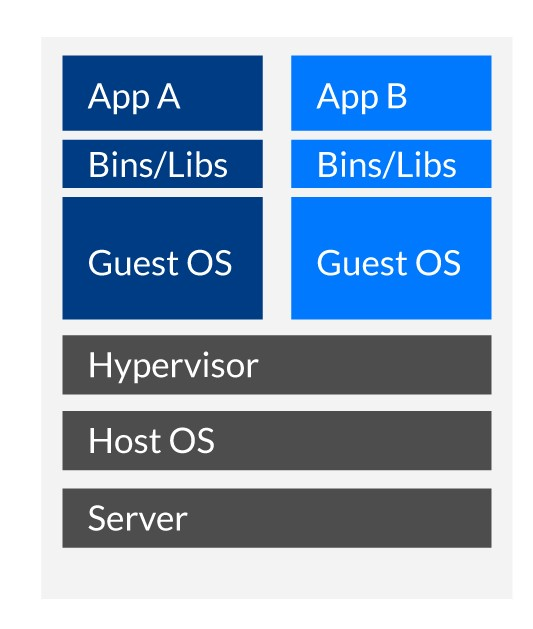
\includegraphics[width=5cm]{./Imagenes/jerarquia1} 
	\end{center}
\end{itemize} 

\begin{itemize}
	\item Jerarquia contenedor
	\\ \textbf{-El servidor o una computador}.
	\\ \textbf{-El sistema operativo} que hospeda y administra los recursos del servidor o computador.
	\\ \textbf{-Docker Engine} virtualizacion a nivel del sistema operativo permite multiples instancias aisladas.
	\\ \textbf{-Bins/Libs} Binarios y librerias.
	\\ \textbf{-App} Aplicacion a ejecutar.
	\begin{center}
	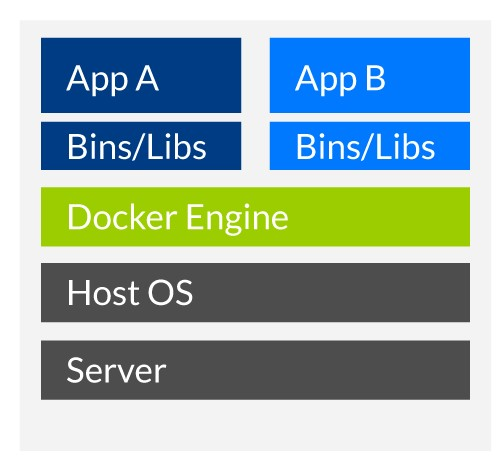
\includegraphics[width=5cm]{./Imagenes/jerarquia2} 
	\end{center}
\end{itemize} 

\begin{itemize}
	\item Los contenedores permiten desplegar aplicaciones más rápido, arrancarlas y pararlas más rápido y aprovechar mejor los recursos de hardware.
	\item La solución de virtualización permite gestionar de forma centralizada los sistemas virtualizados así como sus recursos de almacenamiento:
	\item Reducción de los costes de IT gracias al aumento de la eficiencia y la flexibilidad en el uso de recursos.
	\item Administración global centralizada y simplificada.
	\item Mejora en los procesos de clonación y copia de sistemas: Mayor facilidad para la creación de entornos de test que permiten poner en marcha nuevas aplicaciones sin impactar a la producción, agilizando el proceso de las pruebas.
	\item Aislamiento : un fallo general de sistema de una máquina virtual no afecta al resto de máquinas virtuales.



\end{itemize} 

\section{Concluciones}

Lorem Lorem lorem lorem lorem. 
\begin{itemize}
\item Donec dolor arcu, rutrum id molestie in, viverra sed diam
\item Curabitur feugiat
\item turpis sed auctor facilisis

\end{itemize}
%----------------------------------------------------------------------------------------
%	REFERENCE LIST
%----------------------------------------------------------------------------------------

\begin{thebibliography}{99} % Bibliography - this is intentionally simple in this template

\bibitem[Figueredo and Wolf, 2009]{Figueredo:2009dg}
Figueredo, A.~J. and Wolf, P. S.~A. (2009).
\newblock Assortative pairing and life history strategy - a cross-cultural
  study.
\newblock {\em Human Nature}, 20:317--330.
 
\end{thebibliography}

%----------------------------------------------------------------------------------------

\end{document}
